\documentclass[11pt,letter,english]{article}
\usepackage{amssymb,babel,colortbl}
\usepackage{hyperref,rotating}
\usepackage{multirow}
\usepackage{color}
\usepackage{amsmath}
\providecommand{\href}[2]{#2}

\oddsidemargin=0mm
\evensidemargin=0mm
\textwidth=160mm
%\textwidth=170mm
%\textheight=232mm
\textheight=9.4in
%\textheight=287mm
\hoffset=0.5cm
%\hoffset=-1.6cm
%\voffset=-0.8cm
\voffset=-2.5cm
%\voffset=-2.4cm
%\documentclass[11pt,letter,english]{article}
%\usepackage{amssymb,babel,colortbl}
%\providecommand{\href}[2]{#2}   
%
%\oddsidemargin=0mm
%\evensidemargin=0mm
%\textwidth=160mm
%\textheight=9.4in
%\hoffset=-0.5cm
%\voffset=-1.2cm

\renewcommand\refname{Bibliography}  

\begin{document}
\nocite{*} 

\small
\newcommand*{\data}{\ifcase\month\or
  January\or February\or March\or April\or May\or June\or
  July\or August\or September\or October\or November\or December\fi
  \space\number\day th,\space\number\year}
%===============================================================================
% New Commands and Definitions
%===============================================================================
\newcommand{\blue}    {\color[named]{Blue}}
\newcommand{\black}   {\color[named]{Black}}
\newcommand{\red}     {\color[named]{Red}}
\newcommand{\green}   {\color[named]{Green}}
\newcommand{\orange}  {\color[named]{Orange}}
\newcommand{\yellow}  {\color[named]{Yellow}}
\newcommand{\magenta} {\color[named]{Magenta}}
\newcommand{\cyan}    {\color[named]{Cyan}}

\def\CP{{\sffamily CP}}

%===============================================================================
% Title
%===============================================================================
\begin{center}
 \section*{\huge{PS-Booster Ejection Correction Dipoles}} 
% \large \textbf{}
 \vspace {0.6cm}
\end{center}

%===============================================================================
% List Of Magnets
%===============================================================================
\subsection*{Goal}

Attempt to reproduce the results in http://wwwpsco.cern.ch/private/gm/gmdescrip/LINC-Note.pdf

\begin{itemize}
\item{Used the latest configuration files for {\bf Ring 3} from Vivien for the ring}
\item{{\bf Matched the optics in MADX (32 bits)} to get the tunes}
\item{After add a horizontal or vertical kick from one of the correction dipoles}
\item{Extract the geometrical relations between the kicks at the entry point and at the center of the ejection Septum, SMH15L1}
\item{Trying different tunes and configurations}
\end{itemize}



%===============================================================================
% Head-to-head Comparison
%===============================================================================
\subsection*{Head-to-head Comparison}

\begin{itemize}

\item Configuration 1: {\bf Expected from Note}
  \begin{itemize}
  \item center of DHZ,DVT 4L1   at=1.327-0.426 m = 0.901 m 
  \item center DHZ,DVT 11L1     at=1.327-0.950 m = 0.377 m 
  \item entrance of SMH15L1 4L1 at=1.327-0.800 m = 0.527 m 
  \end{itemize}

\item Configuration 2: {\bf 2014 Corrected using Tobias' measurements}
  \begin{itemize}
  \item center of DHZ,DVT 4L1   at=1.3355(original)\textcolor{red}{-0.4255(correction)} m = 0.910 m 
  \item center DHZ,DVT 11L1     at=0.296(original) \textcolor{red}{+0.0720(correction)} m = 0.368 m 
  \item entrance of SMH15L1 4L1 at=.909892(center)-0.508706(center$\to$beginning blade) m = 0.401186 m 
  \end{itemize}

\end{itemize}


With the entrance of the septum we understood the beginning of the SMH15L1
septum blade.  From the drawing (thanks to M. Houricane), the blade does not
appear to be centered simmetrically w.r.t. the tank, but slightly shifted
upstream, see sketch in Figure~\ref{fig:smh15l1_simplified}. We Labeled {\bf A}
the distance between the beginning of the tank and the beginning of the
blade, {\bf B} the blade length, {\bf C} the distance between the end of the
blade and the end of the tank and {\bf X} the distance between the beginning of
the blade and the center of the tank. With some simple math one can deduct that:

\begin{equation}
X = \frac{B+C-A}{2}
\end{equation}

Using the values from drawing PS.CA.98411.1 of A=121.03 mm, B=1000.24 mm and
C=138.21 mm, one obtains X=508.706 mm. Thus if in the configuration expected from
the note one sets the SMH15L1 entrance to be at 0.527 m, this means the center
of SM15L1 is at (0.507+0.508706) m = 1.015706 m.

The results of using these values and a kick of 1 mrad are summarized in Table~\ref{tab:geom_rel}.

\begin{figure}[!hbtp]
  \begin{center}
    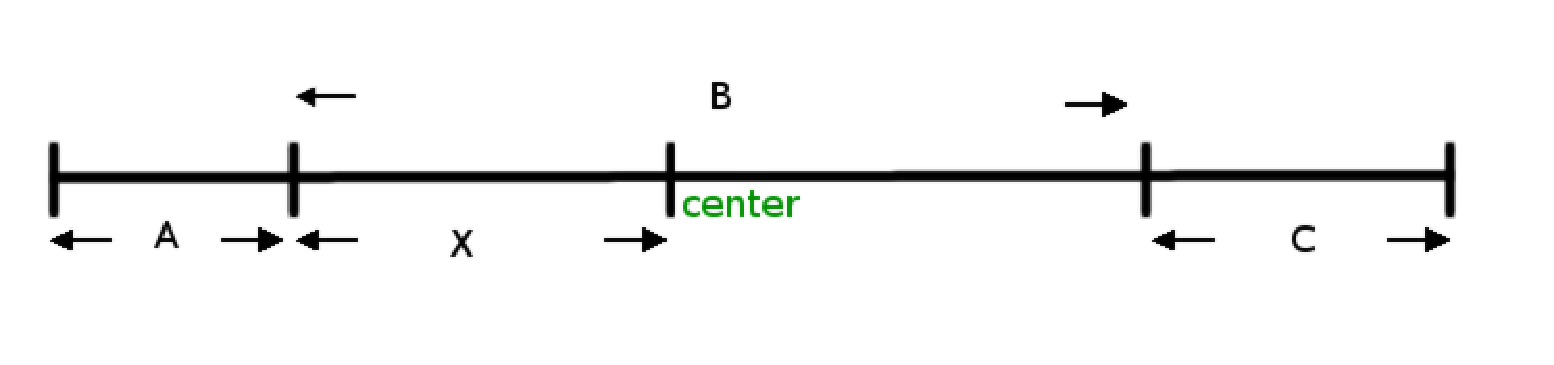
\includegraphics[width=1.0\textwidth]{figs/smh15l1.pdf}
    \caption{simplified drawing of SMH15L1. {\bf A} is the distance between the beginning of the tank and the beginning of the blade. {\bf B} is the blade length. 
      {\bf C} is the distance between the end of the blade and the end of the tank.}
    \label{fig:smh15l1_simplified}
  \end{center}
\end{figure}




\begin{sidewaystable}[h]

  \caption{
    Comparison for the geometrical relation between the kicks in the different PSB sections at the entrance of SMH15L1
    }

  \label{tab:geom_rel}
%\hspace*{-1.3cm}

  \begin{tabular}{ |l|c|c|c|c| }\hline
  Kicker & Note Value               & Config. 1                & Config. 1                & Config. 2               \\ \hline
         & Q$_H$=4.172,Q$_V$=5.230  & Q$_H$=4.172,Q$_V$=5.230  & Q$_H$=4.172,Q$_V$=4.230  & Q$_H$=4.172,Q$_V$=4.230 \\ \hline
         & {\bf entrance of SMH15L1}             & {\bf Beginning Blade}                 & {\bf Beginning Blade}                 & {\bf Beginning Blade}                 \\ \hline

  \multirow{2}{*}{BE3.DHZ4L1} & $\Delta$X$_{ES}$[mm]  = 0.760 $\cdot$ DHZ4L1 [mrad] & 0.786 & 0.768 & 0.641 \\  \cline{2-5}
                              & $\Delta$X'$_{ES}$[mm] = 0.947 $\cdot$ DHZ4L1 [mrad] & 0.938 & 0.937 & 0.938 \\  \hline      
  \multicolumn{5}{|c|}{}        \\ \hline

  \multirow{2}{*}{BE3.DHZ11L1} & $\Delta$X$_{ES}$[mm]  = 5.615 $\cdot$ DHZ11L1 [mrad] & 5.572 & 5.487 & 5.478 \\ \cline{2-5} 
                               & $\Delta$X'$_{ES}$[mm] = 0.104 $\cdot$ DHZ11L1 [mrad] & 0.105 & 0.103 & 0.101 \\ \hline      
 \multicolumn{5}{|c|}{} \\ \hline

 \multirow{2}{*}{BE3.DVT4L1} & $\Delta$Y$_{ES}$[mm]  = -2.122 $\cdot$ DVT4L1 [mrad] & -2.143 & 0.596 & 0.500 \\  \cline{2-5}  
                             & $\Delta$Y'$_{ES}$[mm] =  0.021 $\cdot$ DVT4L1 [mrad] &  0.023 & 0.708 & 0.709 \\  \hline       
 \multicolumn{5}{|c|}{} \\ \hline

 \multirow{2}{*}{BE3.DVT11L1} & $\Delta$Y$_{ES}$[mm]  =  0.669 $\cdot$ DVT11L1 [mrad] &  0.710 & 3.147 & 3.137 \\ \cline{2-5}  
                              & $\Delta$Y'$_{ES}$[mm] = -0.793 $\cdot$ DVT11L1 [mrad] & -0.798 & 0.108 & 0.107 \\ \hline       
 \multicolumn{5}{|c|}{} \\ \hline

\end{tabular}
\end{sidewaystable}


From Figure \ref{fig:BE_DHZ4L1} to \ref{fig:BE_DVT11L1} we report the horizontal
and vertical distortions along the machine circumference resulting from a 1 mrad
kick in the dipoles BE3.DHZ4L1, BE3.DHZ11L1, BE3.DVT4L1 and BE3.DVT11L1,
respectively.


\begin{figure}[!hbtp]
  \begin{center}
    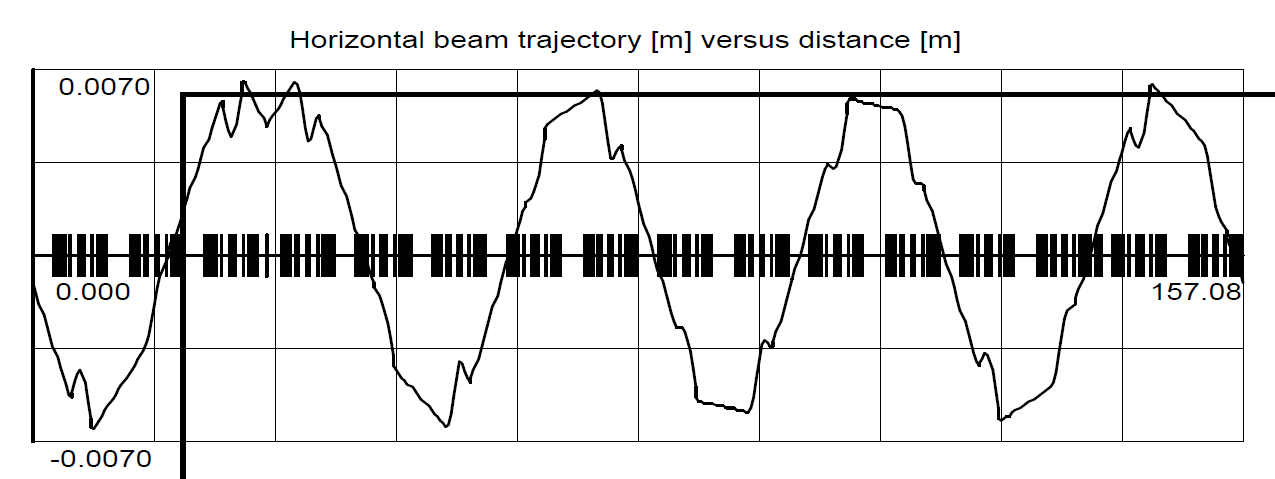
\includegraphics[width=0.8\textwidth]{figs/LINC-BE_DHZ4L1.png}
    %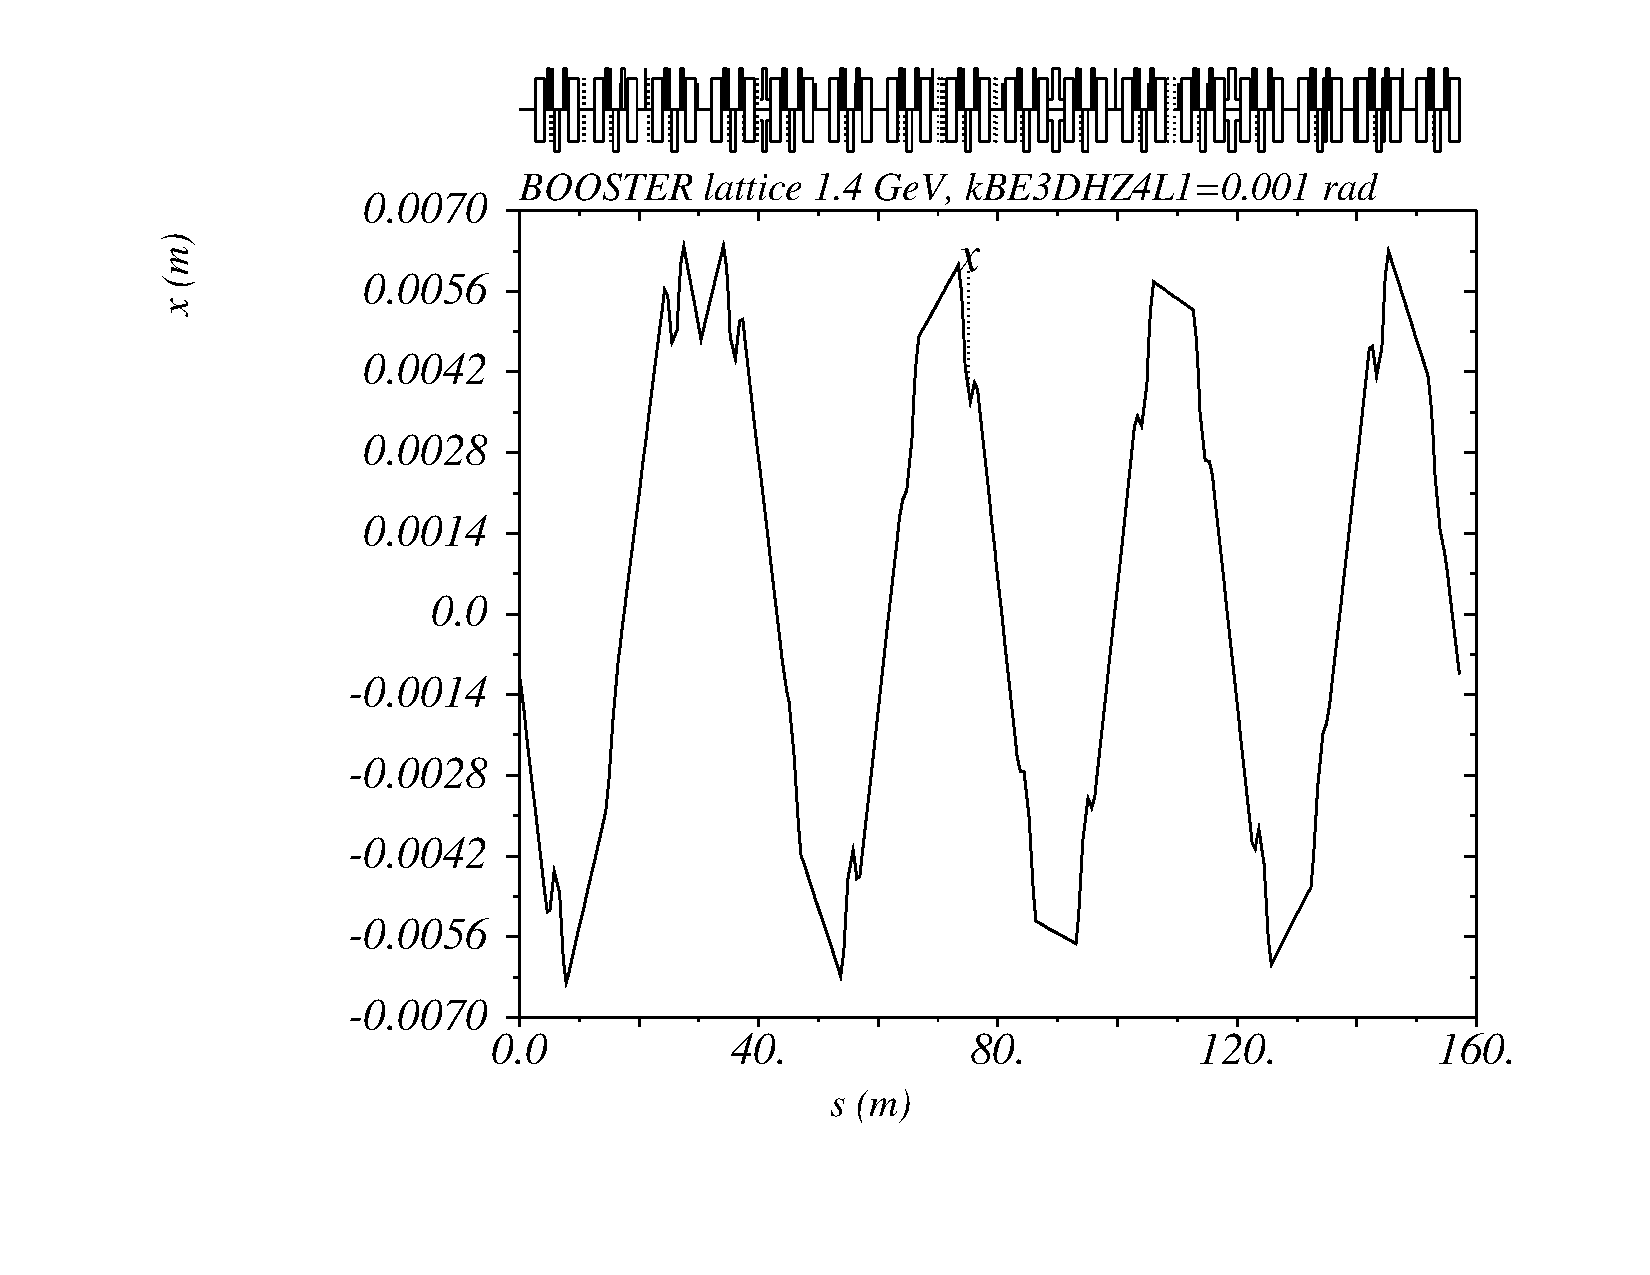
\includegraphics[width=0.8\textwidth]{figs/psb_orbit_kBE3DHZ4L1at0p001rad_lexpfromnote.pdf}
    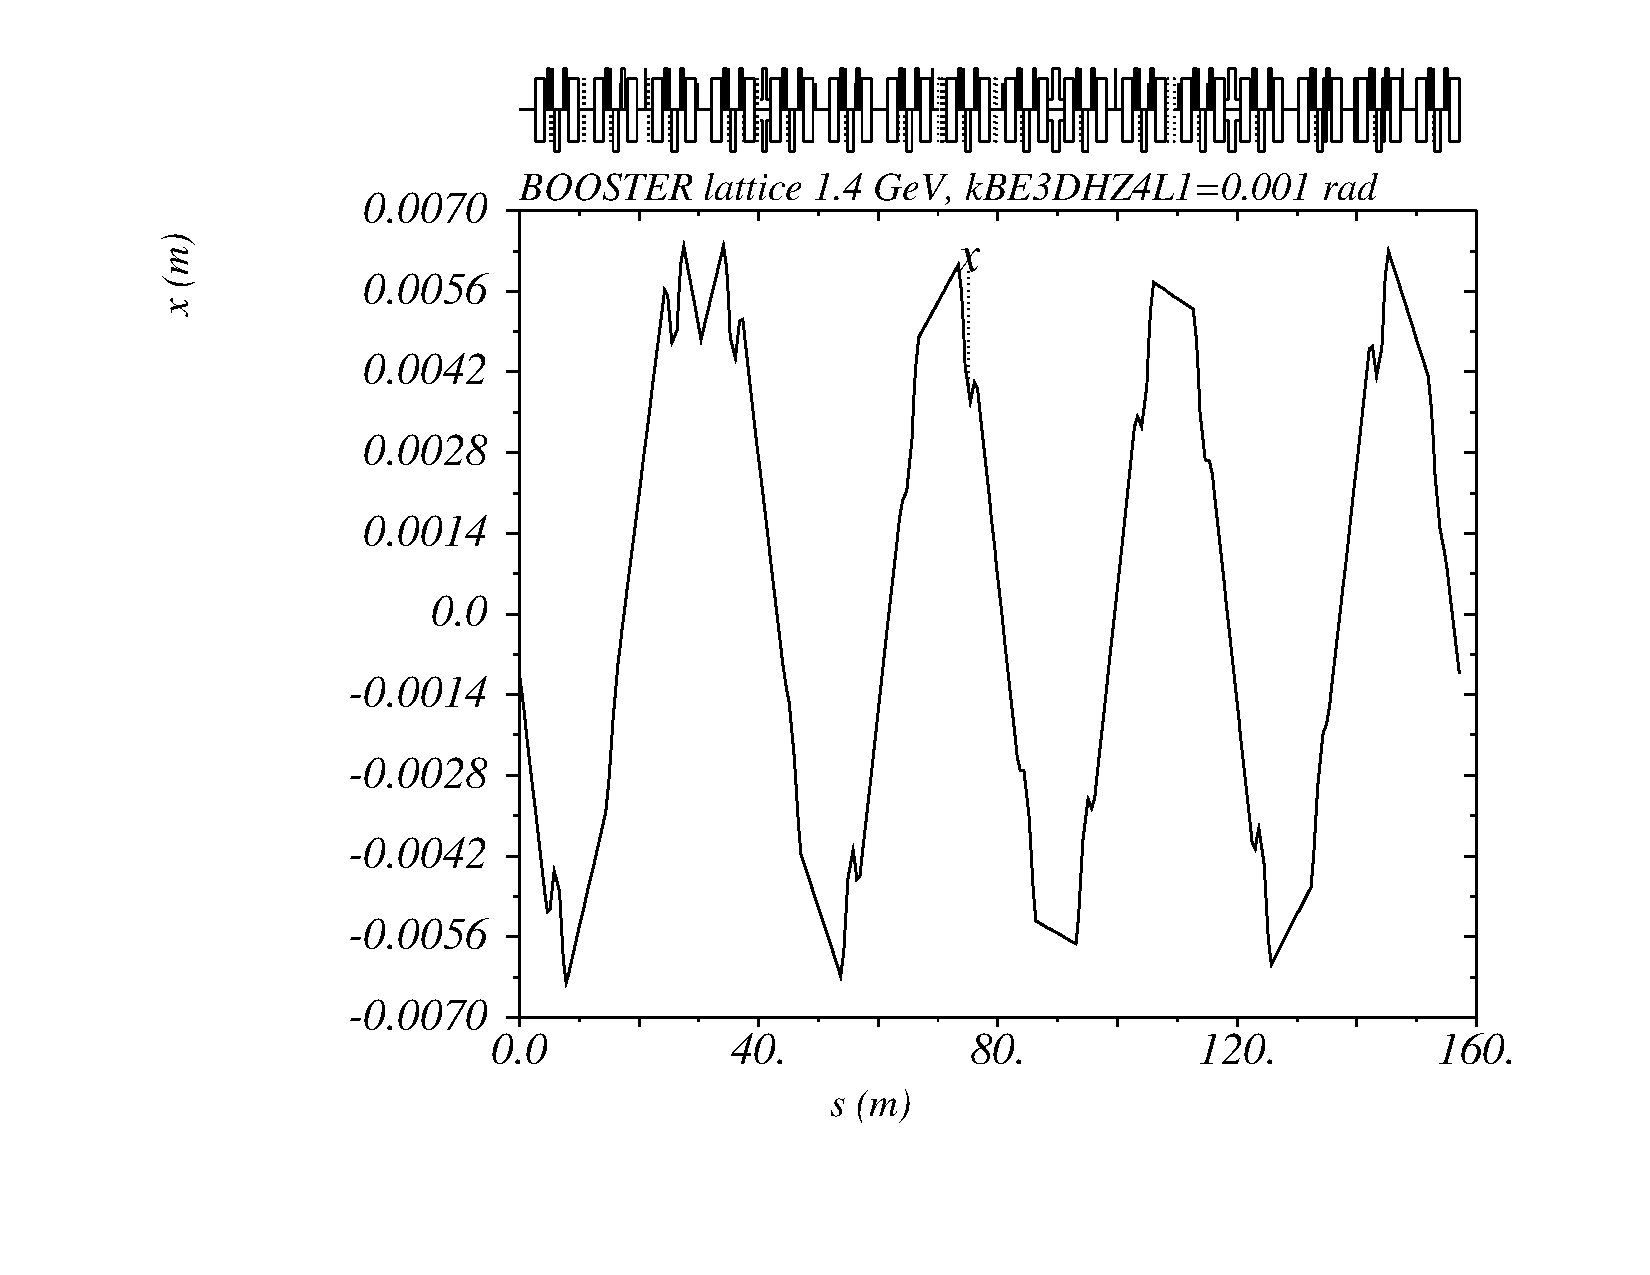
\includegraphics[width=0.8\textwidth]{figs/psb_orbit_kBE3DHZ4L1at0p001rad_l2014tobias.pdf}
    \caption{Closed Orbit comparison for a kick of 1 mrad for BE3.DHZ4L1. Top: Configuration 1, using the tunes Q$_H=4.17$ and Q$_V=5.23$. Bottom: Configuration 2, using the tunes Q$_H=4.17$ and Q$_V=4.23$}
    \label{fig:BE_DHZ4L1}
  \end{center}
\end{figure}


\begin{figure}[!hbtp]
  \begin{center}
    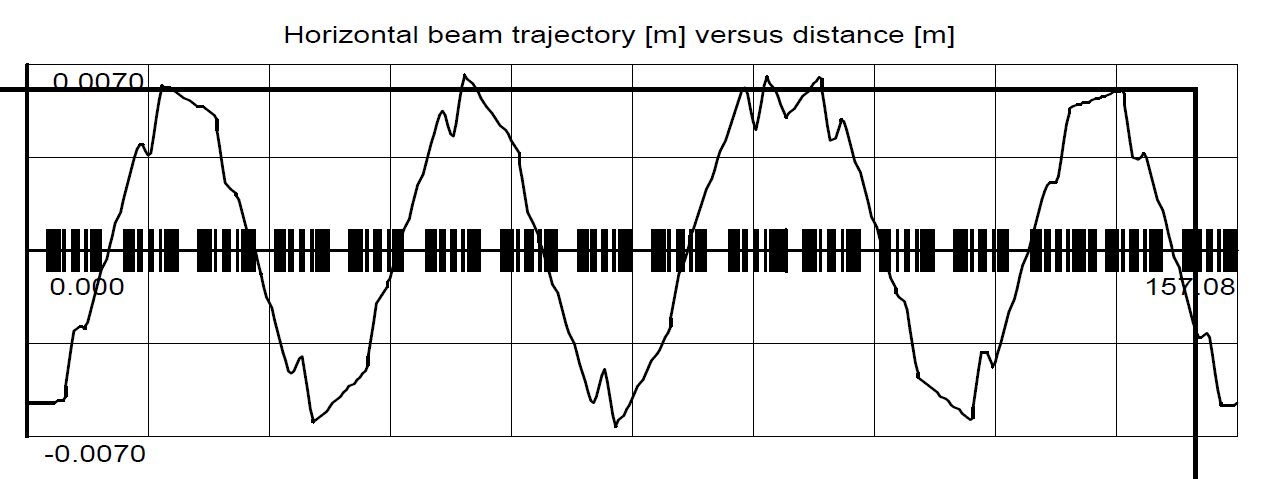
\includegraphics[width=0.8\textwidth]{figs/LINC-BE_DHZ11L1.png}
    %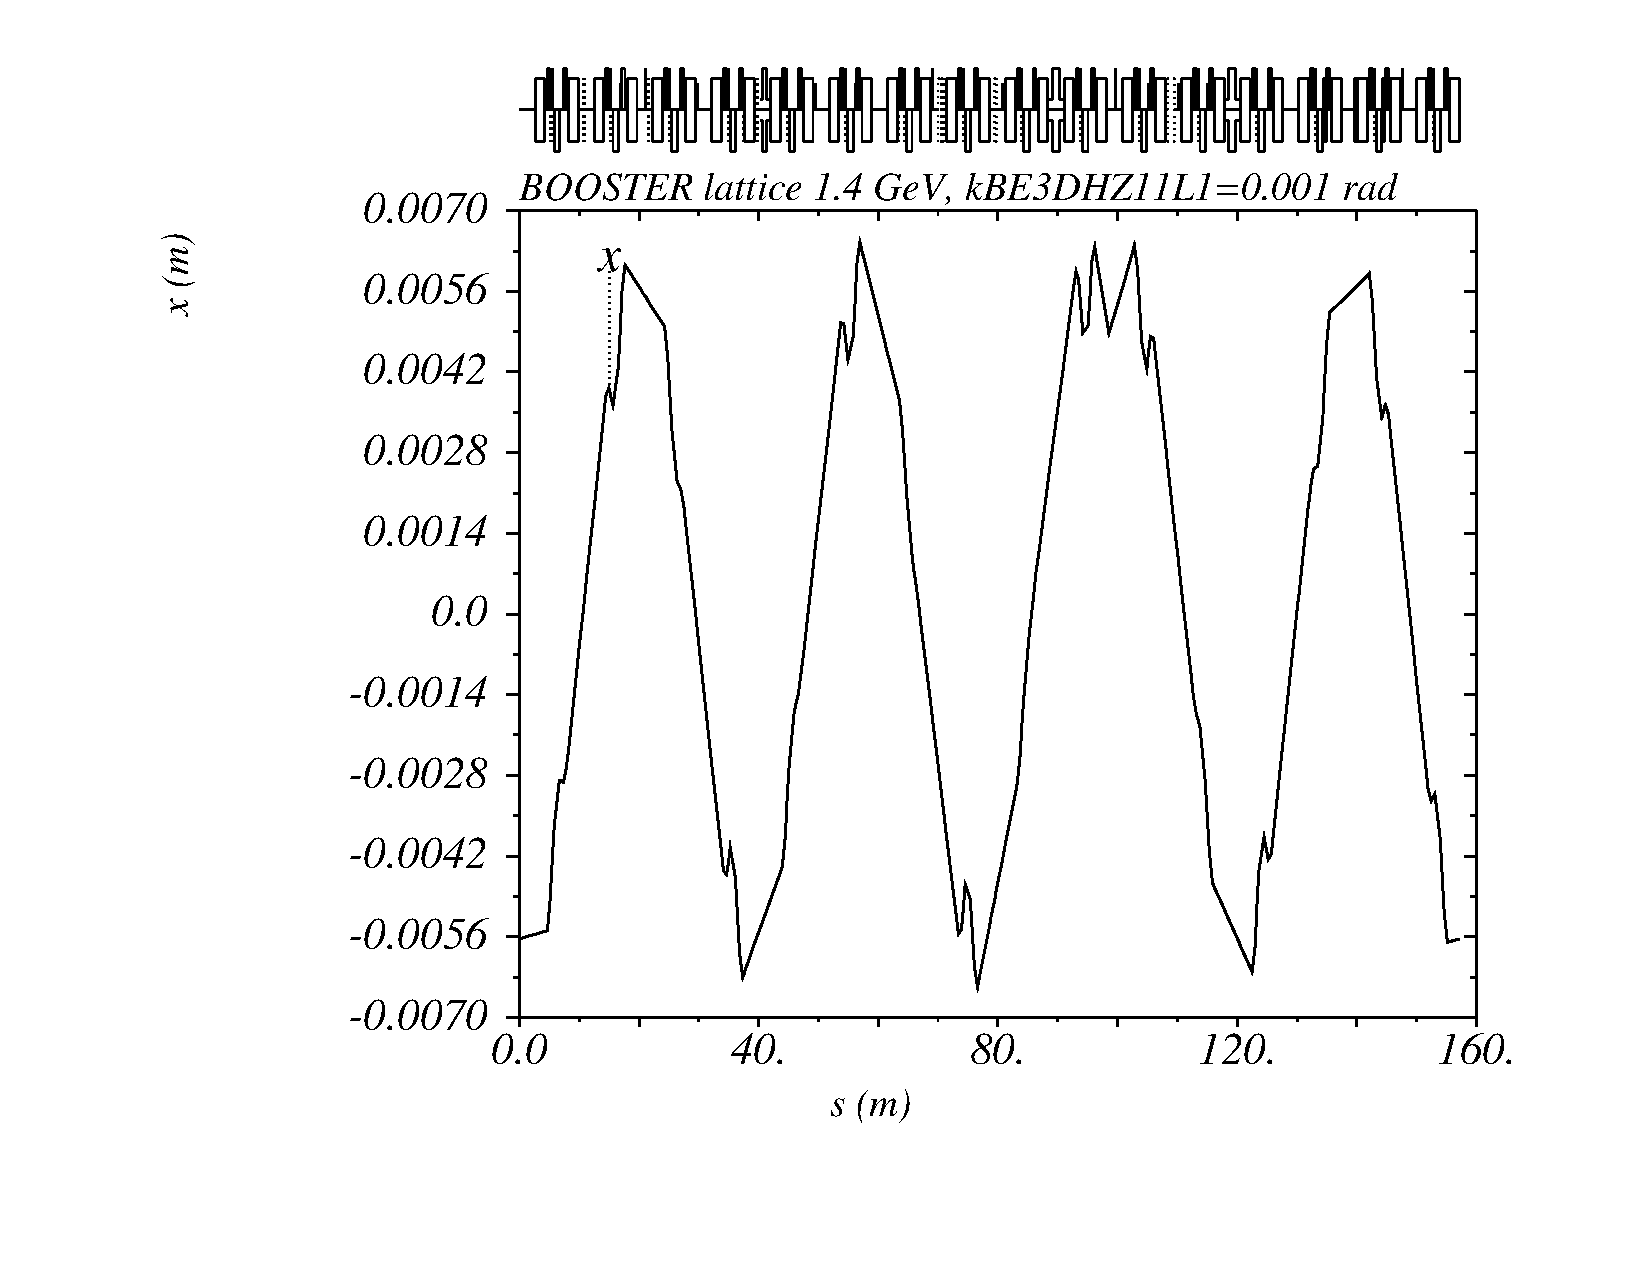
\includegraphics[width=0.8\textwidth]{figs/psb_orbit_kBE3DHZ11L1at0p001rad_lexpfromnote.pdf}
    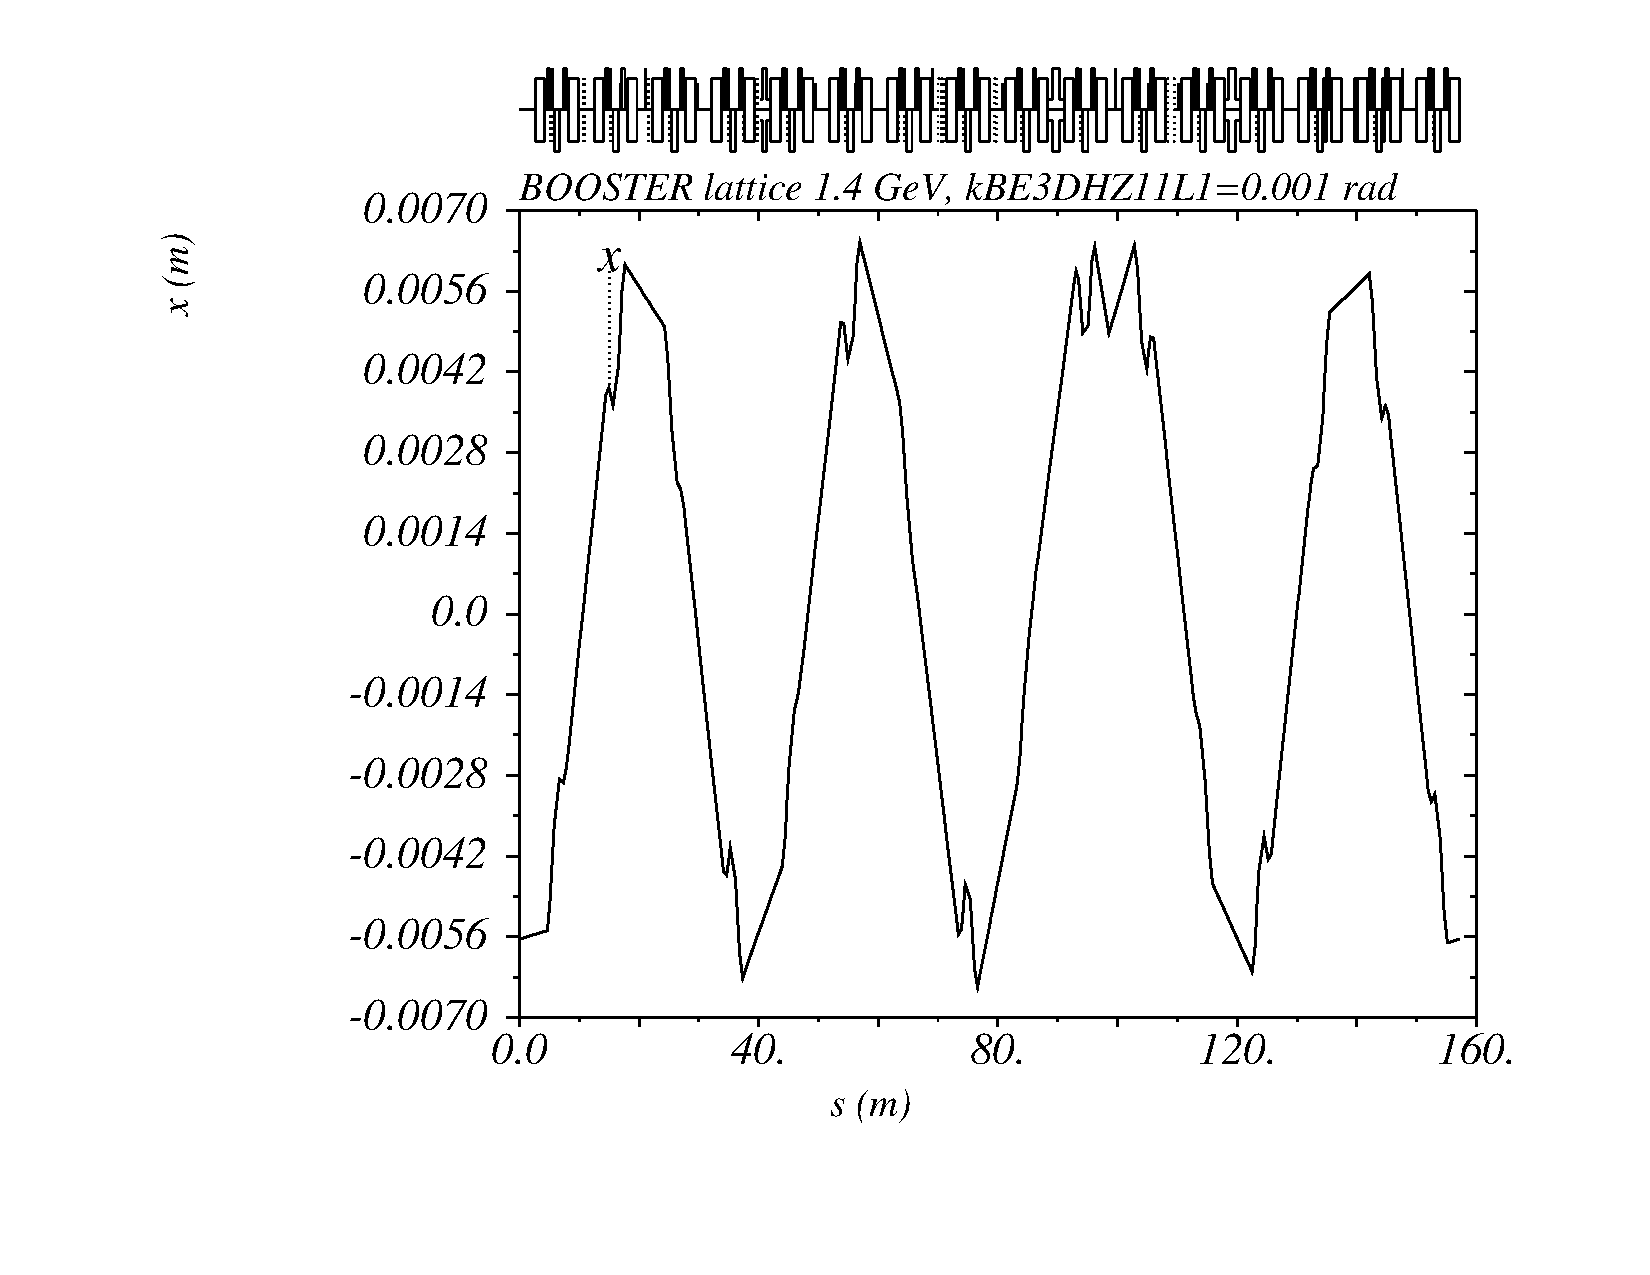
\includegraphics[width=0.8\textwidth]{figs/psb_orbit_kBE3DHZ11L1at0p001rad_l2014tobias.pdf}
    \caption{Closed Orbit comparison for a kick of 1 mrad for BE3.DHZ11L1. Top: Configuration 1, using the tunes Q$_H=4.17$ and Q$_V=5.23$. Bottom: Configuration 2, using the tunes Q$_H=4.17$ and Q$_V=4.23$}
    \label{fig:BE_DHZ11L1}
  \end{center}
\end{figure}



\begin{figure}[!hbtp]
  \begin{center}
    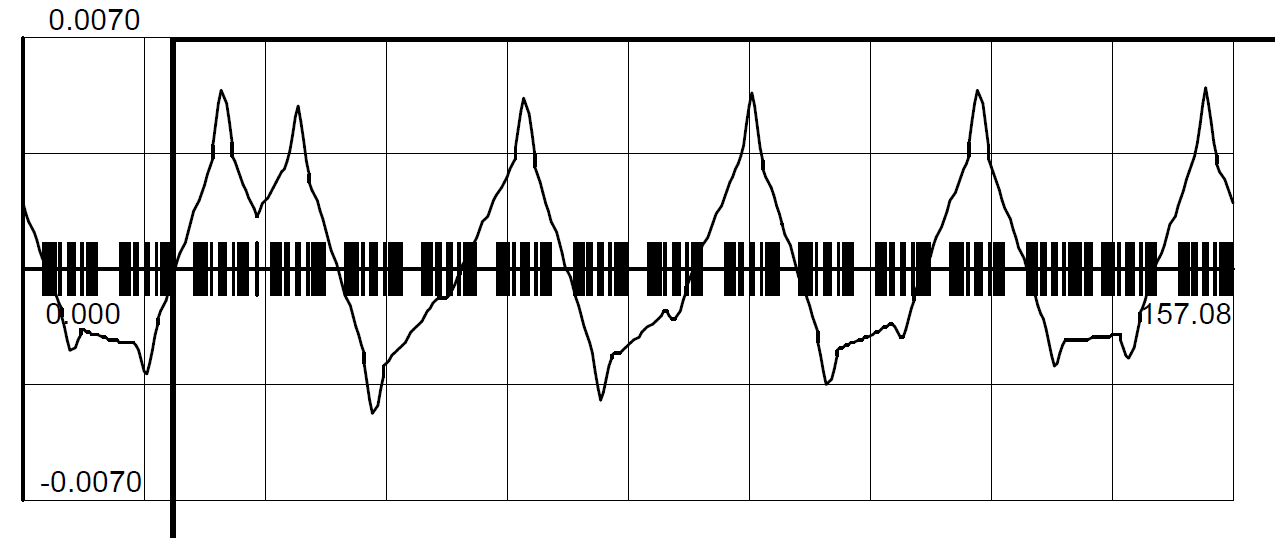
\includegraphics[width=0.8\textwidth]{figs/LINC-BE_DVT4L1.png}
    %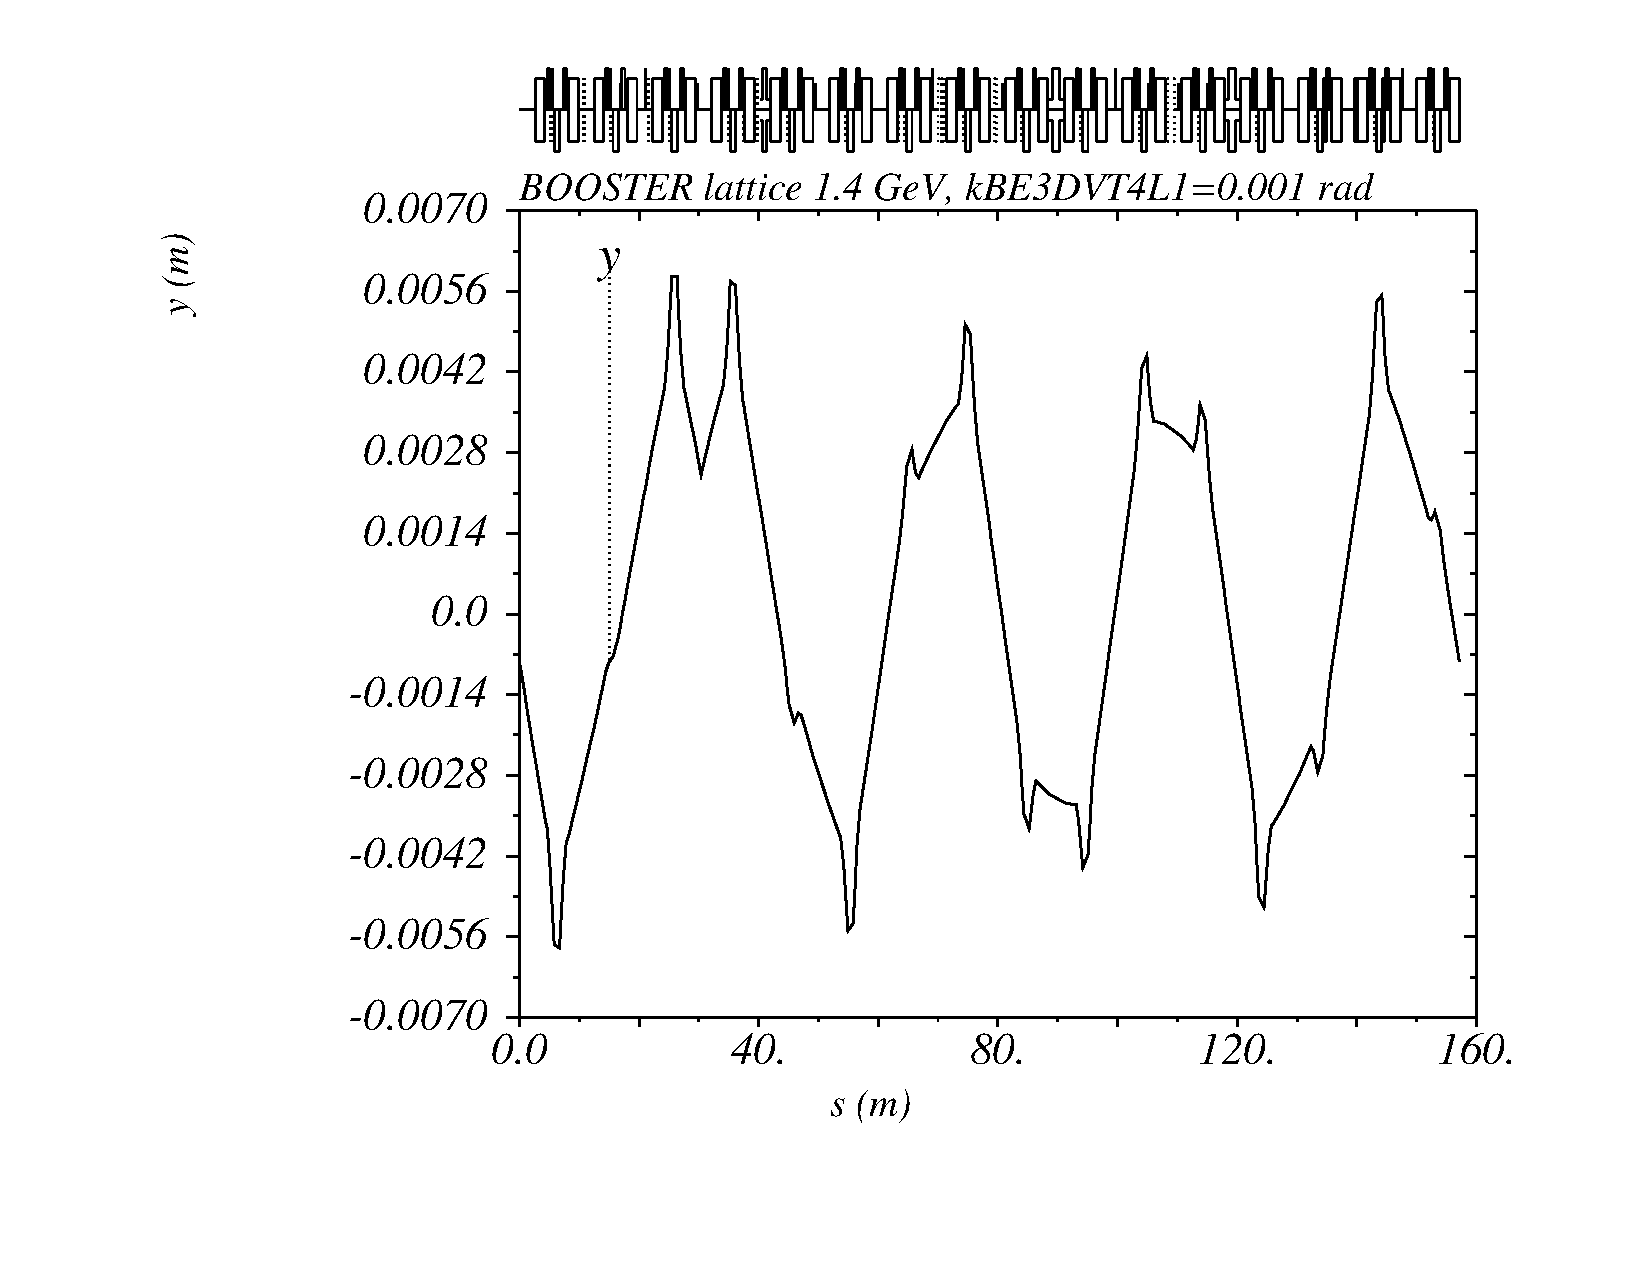
\includegraphics[width=0.8\textwidth]{figs/psb_orbit_kBE3DVT4L1at0p001rad_lexpfromnote.pdf}
    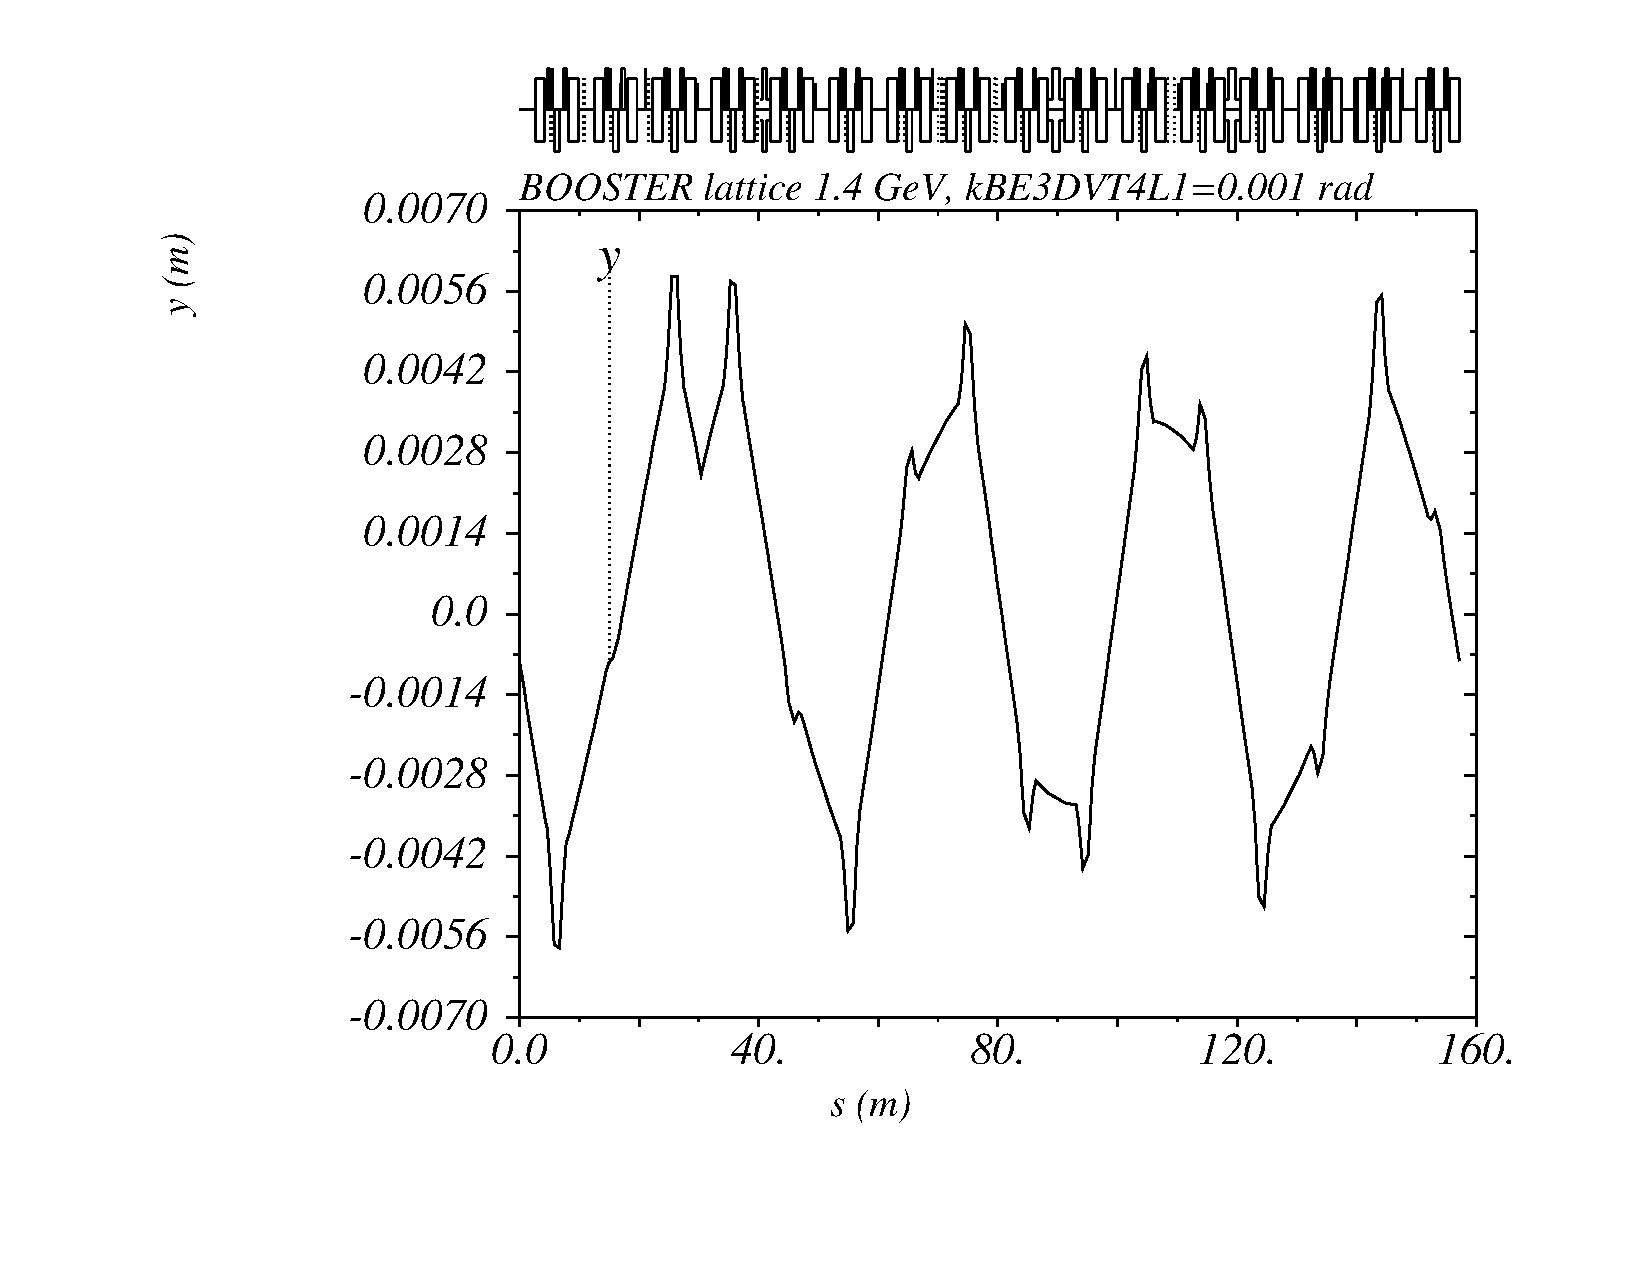
\includegraphics[width=0.8\textwidth]{figs/psb_orbit_kBE3DVT4L1at0p001rad_l2014tobias.pdf}
    \caption{Closed Orbit comparison for a kick of 1 mrad for BE3.DVT4L1. Top: Configuration 1, using the tunes Q$_H=4.17$ and Q$_V=5.23$. Bottom: Configuration 2, using the tunes Q$_H=4.17$ and Q$_V=4.23$}
    \label{fig:BE_DVT4L1}
  \end{center}
\end{figure}


\begin{figure}[!hbtp]
  \begin{center}
    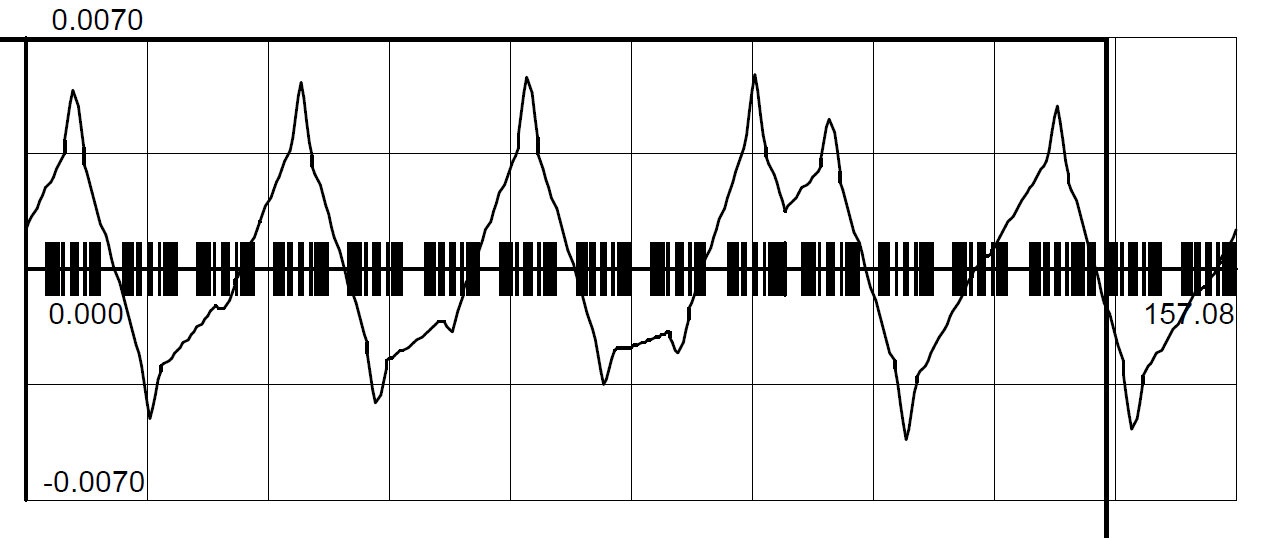
\includegraphics[width=0.8\textwidth]{figs/LINC-BE_DVT11L1.png}
    %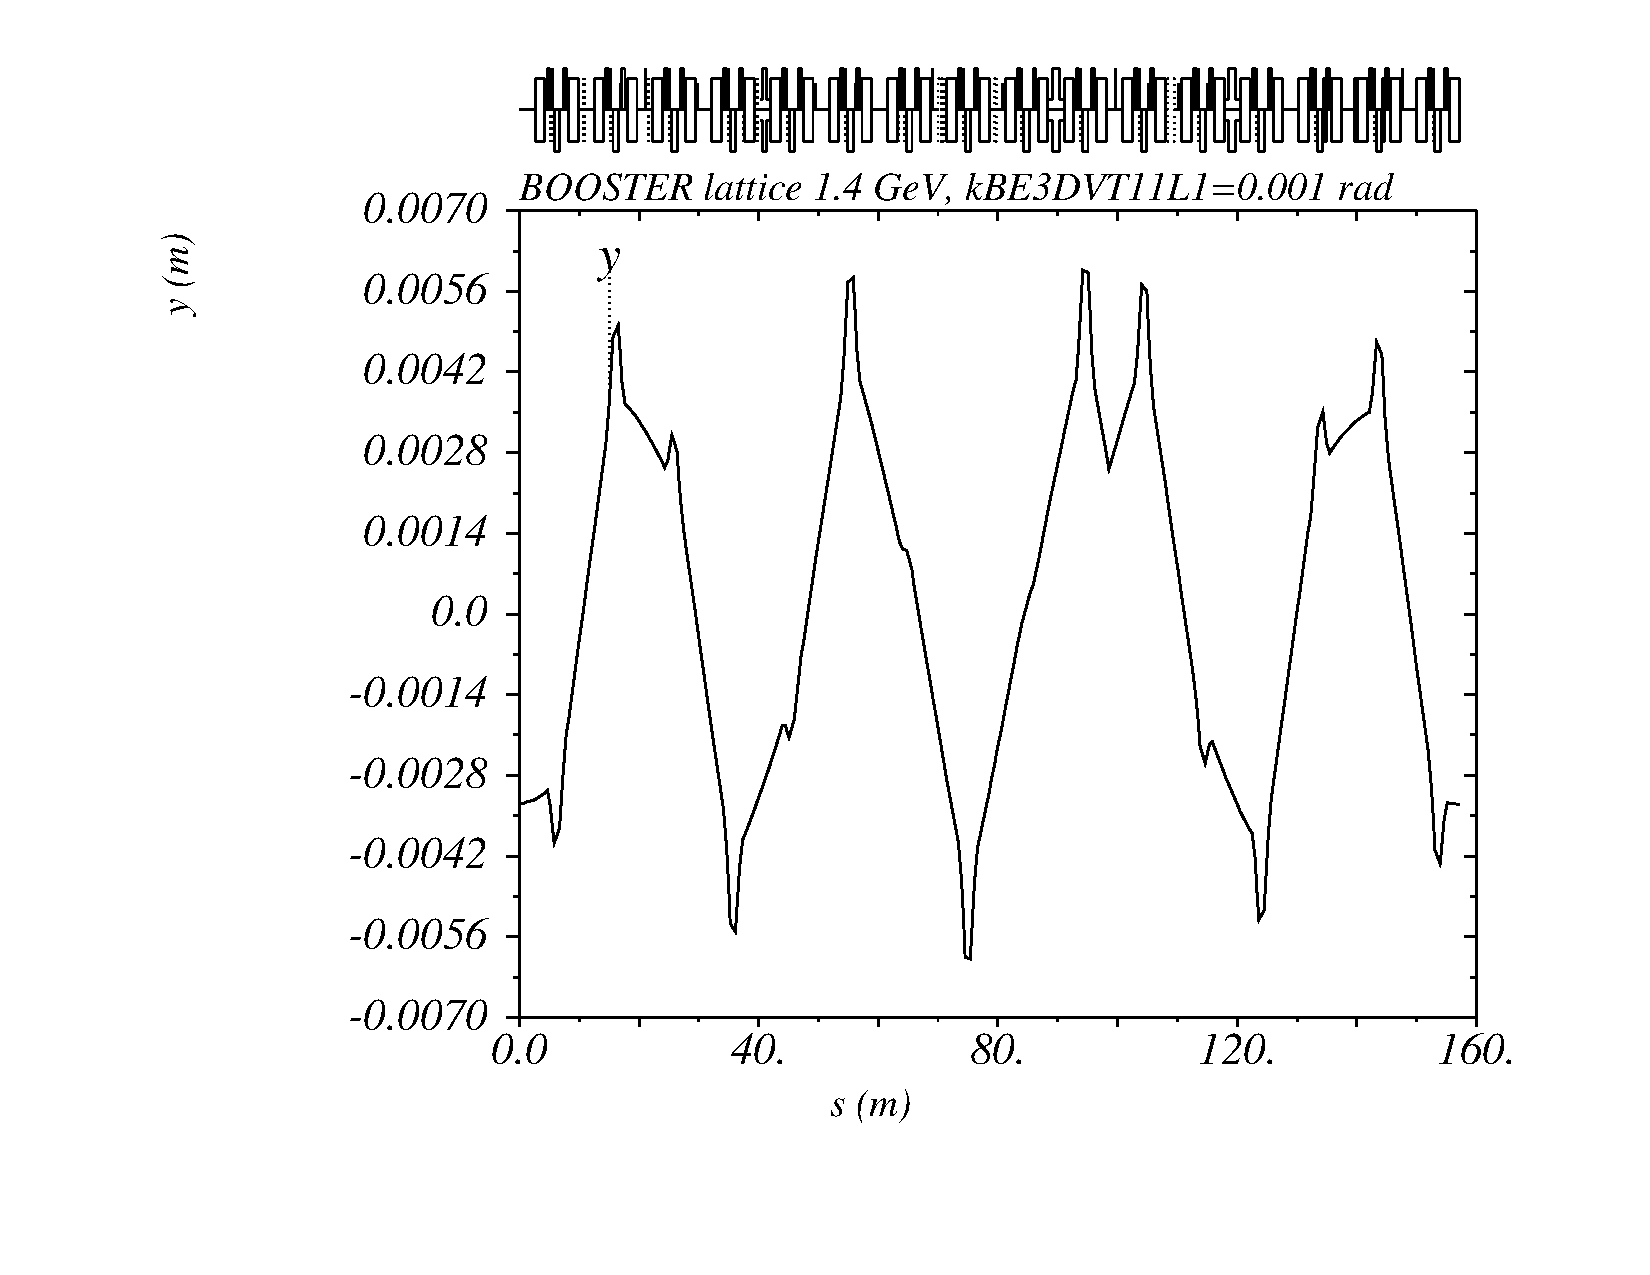
\includegraphics[width=0.8\textwidth]{figs/psb_orbit_kBE3DVT11L1at0p001rad_lexpfromnote.pdf}
    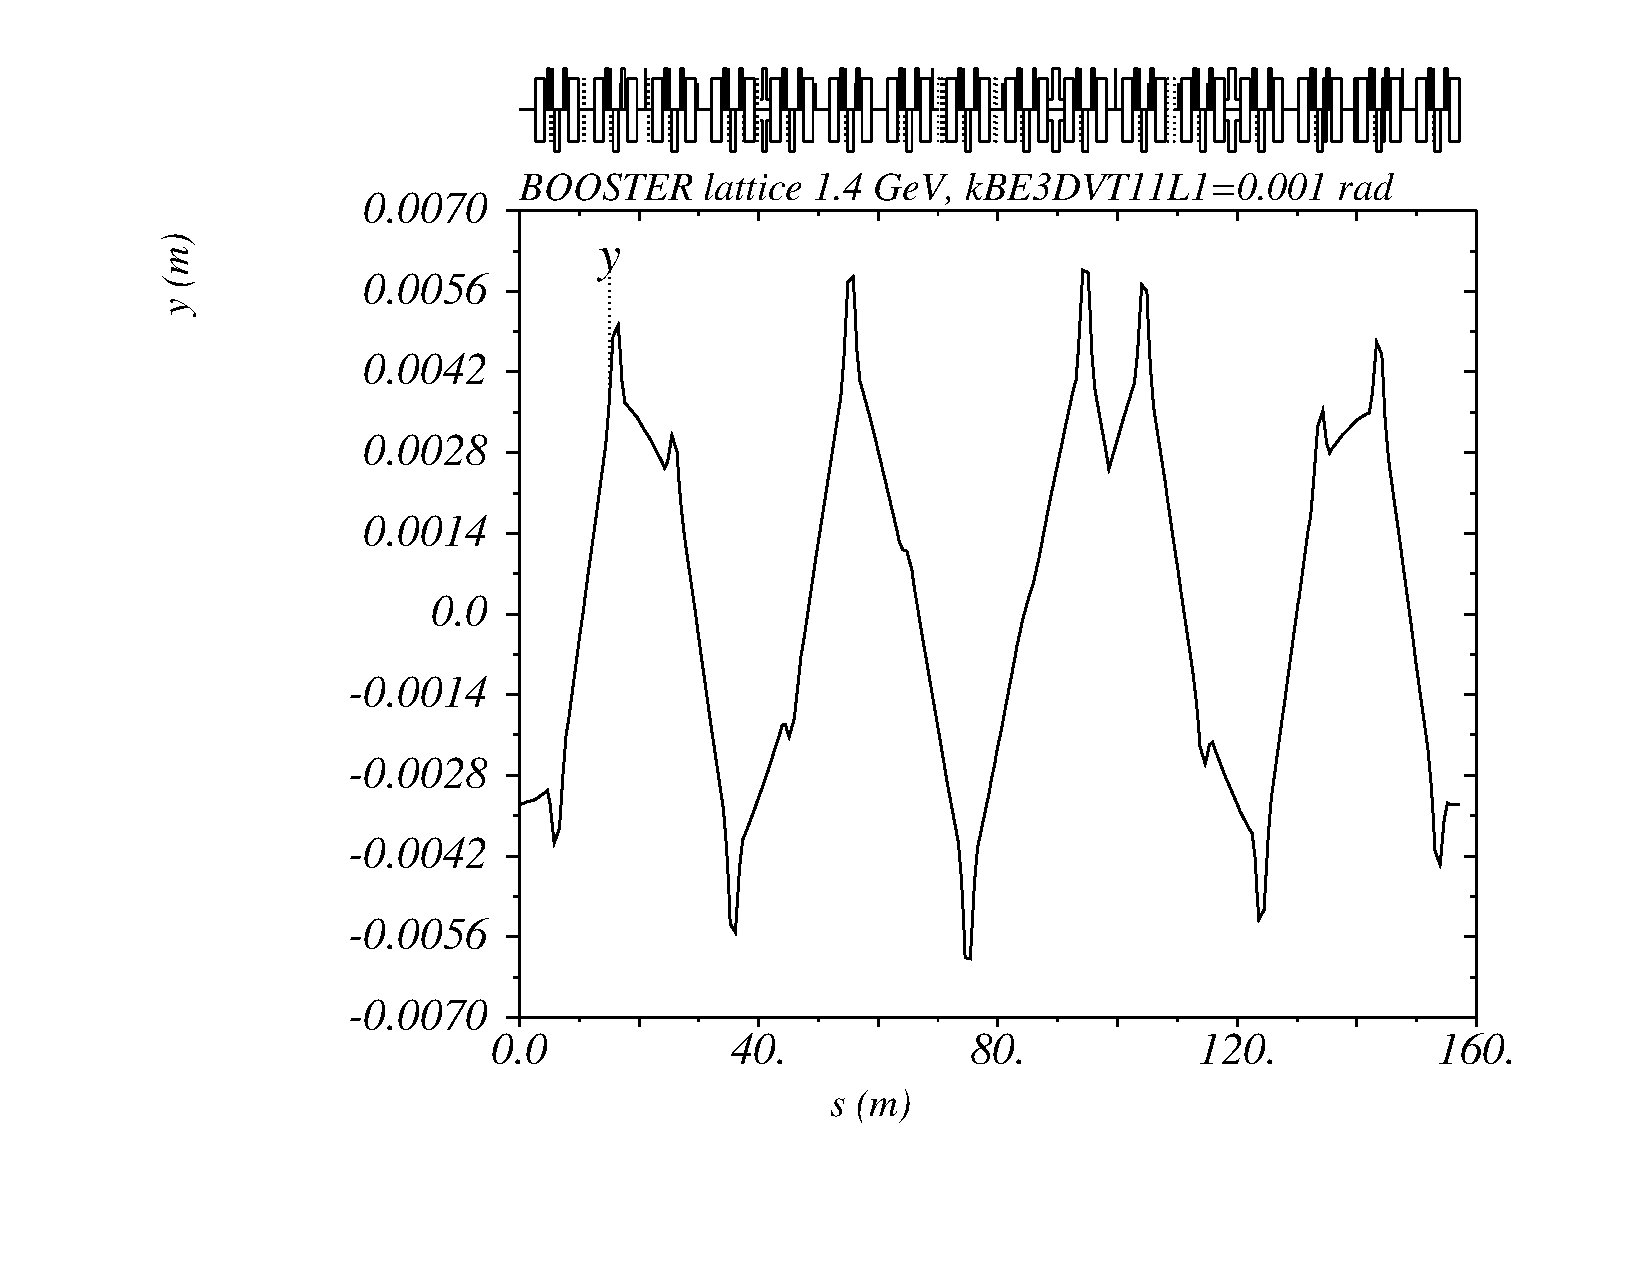
\includegraphics[width=0.8\textwidth]{figs/psb_orbit_kBE3DVT11L1at0p001rad_l2014tobias.pdf}
    \caption{Closed Orbit comparison for a kick of 1 mrad for BE3.DVT11L1. Top: Configuration 1, using the tunes Q$_H=4.17$ and Q$_V=5.23$. Bottom: Configuration 2, using the tunes Q$_H=4.17$ and Q$_V=4.23$}
    \label{fig:BE_DVT11L1}
  \end{center}
\end{figure}

\clearpage

The control power supplies and also for the acquisition need the deflection of
each dipole magnet to be expressed in term of its current.
The deflection-per-current factors for a beam energy of 1.4 GeV is measured to be:
\begin{equation}
\frac{\mbox{Deflection}}{\mbox{Current}} = 0.113 \frac{\mbox{mrad}}{\mbox{A}}
\end{equation}

Using this scale factor the newly evaluated geometrical relation can be written as 

\begin{equation}
\left( \begin{array}{c}
\Delta X_{ES}  \mbox{[mm]}   \\
\Delta X'_{ES} \mbox{[mrad]} \end{array} \right) 
=
\left( \begin{array}{cc}
0.0724 & 0.6190   \\
0.1059 & 0.0114  \end{array} \right) 
\times
\left( \begin{array}{c}
\mbox{DHZ4L1 [A]}   \\
\mbox{DHZ11L1 [A]}  \end{array} \right) 
\end{equation}

\begin{equation}
\left( \begin{array}{c}
\Delta Y_{ES}  \mbox{[mm]}   \\
\Delta Y'_{ES} \mbox{[mrad]} \end{array} \right) 
=
\left( \begin{array}{cc}
0.0565 & 0.3544   \\
0.0801 & 0.0120  \end{array} \right) 
\times
\left( \begin{array}{c}
\mbox{DVT4L1 [A]}   \\
\mbox{DVT11L1 [A]}  \end{array} \right) 
\end{equation}

\end{document}


